
\chapter{Sentiment Classification}
This chapter describes the experiments done. High level description and
execution of experiments. Detailed descriptions of execution and technical
details in appendix. 

Sections in this chapter are as follows. Manual classifications,
\label{sentiment:manual_classification}, where we see how people classify
tweets. Then we count words with 'Word count classification',
\label{sentiment:word_count_classification}. Expanding with the use of
classifiers in section \label{sentiment:classifier_classification}. A
comparison of the classifiers and associated results can be found in section
\label{sentiment:comparison_results}. And a brief discussion an comments come
last, \label{sentiment:comments_discussion}.

%what is sentiment
Sentiment is described as "an attitude toward something; regard;
opinion."\footnote{ Dictionary.com on Sentiment:
\url{http://dictionary.reference.com/browse/sentiment?s=t}}. The sentiment is the perceived positivity of the message that the user tries to
communicate. Sentiment is in many cases a personal thing, and can change from
person to person or from setting to setting. We think of the sentiment as
conveyed meaning of a message. 

%why do we get it
Some of the motivation for acquiring the sentiment of a tweet or a sentence, is
that we can say something about a persons state of mind and from that predict
behaviour. We want to use the sentiment to make smart decisions later. As an
example of usage it would be ideal to find a correlation between sentiment and
stock exchange, thus making us able to increase revenue with decisions
based on the sentiment. 

%how do we use it
In this thesis we have two main ways of classifying tweets. Word counting and
training a classifier. Both methods require dictionaries of positive and
negative words, \ref{data:dictionaries}. In the classifier we use the dictionary
to extract features from a tweet. And with the word counting we count the
number of positive and negative words. 

\section{Manual Classification}\label{sentiment:manual_classification}
When labeling tweets manually there are a number of factors the complicates the
process. Among them are the quality of the tweet, state of mind, language, and
political affiliation.

The quality of the tweet describes the content in many ways. Does the tweet
contain links or hashtags? Are users mentioned?

State of mind for a person dictates that persons actions in many cases. This
also has an effect on labeling tweets. A positive state of mind classifies more
tweets negative as positive then others.

Political affiliation plays a huge role when labeling the obama tweet set. Do
you like obama? Do you like Romney? Neither? This matters. The tweetset in
itself is pro obama. So while labeling this tweet set we put aside political
influence and looked at the core of the sentiment.

Note that all this happens in the brain during 3 to 60 seconds while reading
the tweet text and is a very rough description of the thoughts happening.
Labeling a tweet follows this algorithm in many ways:

\begin{tabular}{ l p{5cm} p{7cm} }
Step & Thought & Description \\
1 & Have we seen this tweet before? & Skip it or use previous classification. \\
2 & \#Hashtags or links present? & Some hashtags are automatically positive or
negative. Also remove noise such as users and links.\\
3 & Sarcasm? & If sarcasm is present, put up a warning flag saying that it is
the opposite of step 4.\\
4 & Special words? & Find a word that triggers positive or negative
impression.\\
5 & Done & Label tweet as positive or negative.\\
\end{tabular}

\paragraph{Result files}
\hspace{0pt}\\
When classifying with manually we create files with the results. These files
are comma separated files with three fields.
\begin{itemize}
    \item Sentiment: Positive, neutral or negative. Represented by 1, 0 or -1.
    \item Tweet id, if it exists, else 'id'. It is a long number.
    \item The tweet text. In some cases sanitized.
\end{itemize}

\paragraph{Obama tweet set}
\hspace{0pt}\\
When labeling the obama tweet set we found that the tweets present was rather
rubbish. Whether or not the data is representative for twitter in general is
difficult to say. But we observed lots of retweets and political related
content. Tweets favoring obama are positive for poeple who support obama and
negative for supporters of Romney at the same time. So while labeling the
tweets we tried to remove personal political views from the equation, but that
is very difficult in the long run.  

\paragraph{Kiro tweet set}
\hspace{0pt}\\
The kiro tweet set also has a lot of retweets, but they are not use later,
thereby removing the retweet reduced data uniqueness. Also the search terms the
dataset is based on could be broader to increase the spectrum of tweets.  
%

\section{Word count classification}\label{sentiment:word_count_classification}
We describe the classification process and the different parts of it, then we
show the results and discuss the drawbacks of this method. The algorithm does,
simply put, count the positive and negative words. More positive words than
negative means the tweet is positive and vice versa. 

\subsection{Classification}
\paragraph{Polarity} 
\hspace{0pt}\\ 
The polarity of a given tweet is based on the difference in the amount of
positive verses negative words. 

First we calculate the amount of positive words. Then divide that on the total
amount of words. Giving us the percentage of positive words. Then we do the same thing for negative words.

Then we look at the difference between the negative and the positive word
percentage. If the difference is positive we have a positive tweet. And if the
difference is negative we have a negative tweet.

Code wise we get something like this: 
\begin{verbatim}
var positive_words_count
var negative_words_count

positivity = positive_words_count / total_number_words
negativity = negative_words_count / total_number_words

polarity = positivity - negativity

if polarity > 0: 
    tweet is positive
else: 
    tweet is negative
\end{verbatim}

\paragraph{Threshold} 
\hspace{0pt}\\ 
Threshold is the ratio of positive vs negative words that has to be present for a
tweet to be either positive of negative.

The percentage of positive words minus the percentage of negative words gives
the polarity value, or the positivity(how positive a tweet is) of a tweet. 
When actually deciding if a tweet is positive or negative we look at the
polarity value. If the polarity value is above the threshold (polarity >
threshold) the tweet is classified as positive. 

\paragraph{Examples of classification follows:} 
\hspace{0pt}\\ 
Example tweets:
\begin{itemize}
    \item t1 = “good that he was decreasing badly”
    \item t2 = “he was good for increase” 
    \item t3 = “good or bad”
\end{itemize}

Classification of t1:
\begin{itemize}
    \item pos = 1 / 6 = 0.16666
    \item neg = 2 / 6 = 0.33333
    \item polarity = pos - neg = -0.1667
    \item threshold of 0 gives negative classification
    \item threshold of 0.1 gives negative classification
    \item threshold of -0.2 gives positive classification
\end{itemize}

Classification of t2:
\begin{itemize}
    \item pos = 2 / 5 (to av fem ord) = 0.4
    \item neg = 0 / 5 = 0
    \item polarity = pos - neg = 0.4 - 0.0 = 0.4
    \item threshold = 0.4 ⇒ positive
    \item threshold = 0.5 ⇒ negative
    \item threshold = -0.1 ⇒ positive
\end{itemize}

Classification of t3:
\begin{itemize}
    \item pos = 1 / 3 = 0.3333
    \item neg = 1 / 3 = 0.3333
    \item polarity = pos - neg = 0
    \item threshold = 0 ⇒ positive
    \item threshold = 0.1 ⇒ negative
    \item threshold = -0.1 ⇒ positive
\end{itemize}

Further we found the best average threshold value to be 0.1.
From the table under we have the threshold value, and the average
classification accuracy among the 18 entries for each threshold value. 

Average threshold accuracy table:
\hspace{0pt}\\
\begin{tabular}{ c c c c }
Threshold & Accuracy & Threshold & Accuracy \\
- & - & 0.0 & 0.6479 \\
-0.1 & 0.6316 & 0.1 & 0.6516 \\
-0.2 & 0.6161 & 0.2 & 0.6511 \\
-0.3 & 0.6059 & 0.3 & 0.6430 \\
-0.4 & 0.5988 & 0.4 & 0.6305 \\
-0.5 & 0.5888 & 0.5 & 0.6122 \\
-0.6 & 0.5711 & 0.6 & 0.5934 \\
-0.7 & 0.5423 & 0.7 & 0.5712 \\
-0.8 & 0.5083 & 0.8 & 0.5457 \\
-0.9 & 0.4881 & 0.9 & 0.5307 \\
\label{tbl:average_threshold_accuracy}
\end{tabular}

\begin{figure}[htb]
    \centering
    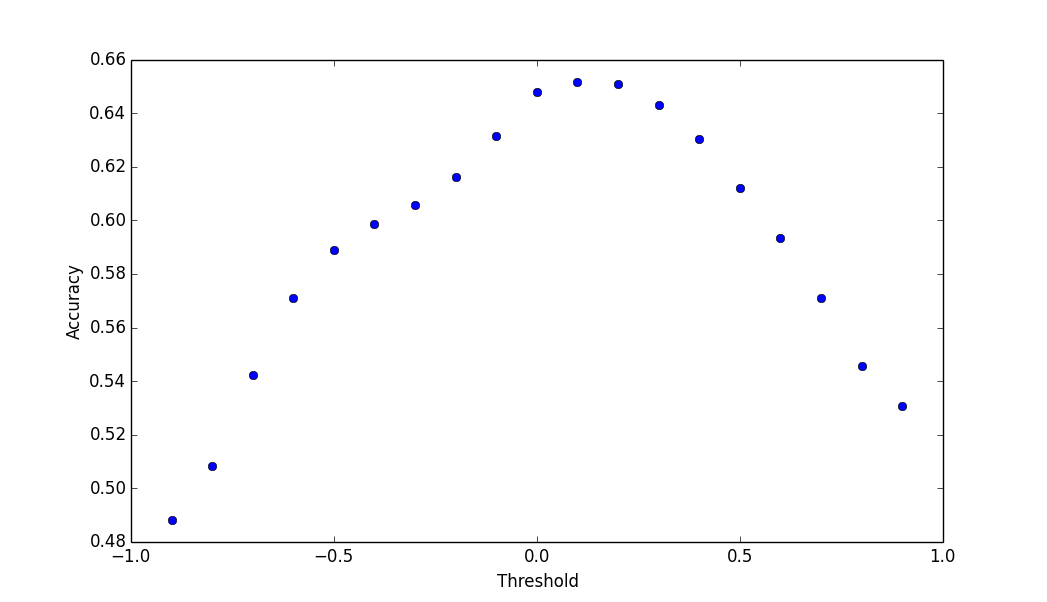
\includegraphics[width=\textwidth]{average_threshold_accuracy.png} 
    \caption{Graph plot of the 'Average threshold accuracy' table.}
    \label{fig:average_threshold_accuracy}
\end{figure}
%

\subsection{Results}
The results from the word count classification can be plotted in the tabled
\ref{tbl:sentiment_word_count_results} and in the graph
\ref{tbl:sentiment_word_count_results}.

\begin{tabular}{ r p{6cm} r r c }
id & Dictionary & Failed & Correct & Accuracy \\
& -- Kiro compiled dataset -- & a & b & b/(a+b) \\
\hline
1 & Monogram, obama & 578 & 419 & 0.4203 \\
2 & Monogram LoughranMcDonald & 491 & 506 & 0.5075 \\
3 & Monogram, combined Obama and LoughranMcDonald & 416 & 581 & 0.5827 \\
4 & Kiro, Monogram, self compiled & 115 & 882 & 0.8847 \\
5 & Kiro, Bigram, self compiled & 17 & 980 & 0.9829 \\
6 & Kiro, Trigram, self compiled & 18 & 979 & 0.9819 \\
7 & Obama, Monogram, self compiled & 567 & 430 & 0.4313 \\
8 & Obama Bigram, self compiled & 534 & 463 & 0.4644 \\
9 & Obama Trigram, self compiled & 567 & 430 & 0.4313 \\

& -- Obama tweet set -- & a & b & b/(a+b) \\
\hline
10 & Monogram, obama & 855 & 510 & 0.3736 \\
11 & Monogram LoughranMcDonald & 508 & 857 & 0.6278 \\
12 & Monogram, combined Obama and LoughranMcDonald & 544 & 821 & 0.6015 \\
13 & Kiro, Monogram, self compiled & 632 & 733 & 0.5370 \\
14 & Kiro, Bigram, self compiled & 521 & 844 & 0.6183 \\
15 & Kiro, Trigram, self compiled & 498 & 867 & 0.6352 \\
16 & Obama, Monogram, self compiled & 493 & 872 & 0.6388 \\
17 & Obama Bigram, self compiled & 37 & 1328 & 0.9729 \\
18 & Obama Trigram, self compiled & 39 & 1326 & 0.9714 \\
\label{tbl:sentiment_word_count_results}
\end{tabular}

5, 6, 17, 18 are the dictionaries with best accuracy. Which is to be expected
for the classification of the dataset the dictionary was created from. 

But more interestingly, if we take the dictionaries created form one dataset,
and look at the results of the classification on the other dataset. We compare
7, 8, 9 with each other and 13, 14, 15 with each other. Then we can see that
the bigram and trigram dictionaries perform overall better than the monogram
dictionaries. 

Further we see indications that the quality of the dictionary plays an
important role. The LoguhranMcDonald monogram dictionary performs quite good
with both datasets. Even on par with the compiled dictionaries on opposite
dataset. This indicates that a well crafted dictionary can perform as well
as compiled dictionaries.  

\begin{figure}[htb]
    \centering
    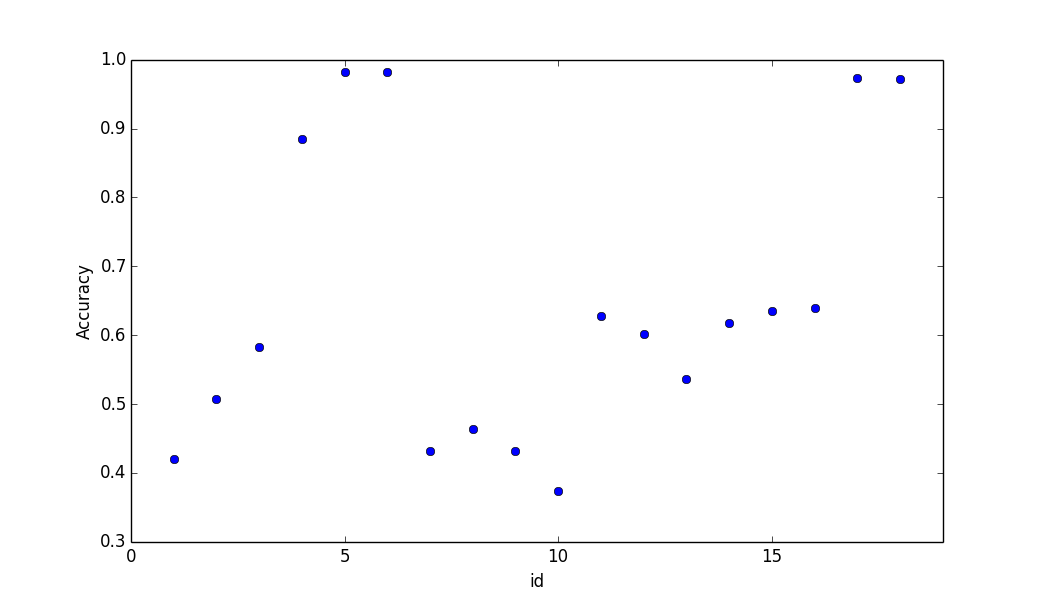
\includegraphics[width=\textwidth]{dictionary_accyracy.png} 
    \caption{The graph shows the plotted accuracies from the word count
classification. The ids represents the ids from the table above,
\ref{tbl:sentiment_word_count_results}}
    \label{fig:dictionary_accyracy}
\end{figure}
 
When comparing the results from one dataset to the other we can see indications
of how the content of the dataset also plays a huge role in the results. Some
tweets are more difficult to classify then others. 
%

\paragraph{Threshold variations}
\hspace{0pt}\\
By varying the threshold we hoped to find an optimal point of which we could
separate tweets based on polarity. From the following
graphs, figure \ref{fig:threshold_graphs}, we can see no clear distinction of
one value being better than the other ones.  

In figure \ref{fig:threshold_graphs} we list the results of the experimentation
with the threshold. Table \ref{tbl:dictionary_to_threshold} lists the
dictionaries and dataset used for which graphs in figure \ref{fig:threshold_graphs}.
'kiro dataset' and 'obama dataset' columns tells which dataset that was
classified in which graph.

\begin{tabular}{ l c c }
\hspace{0pt}\\
Dictionary name and description & kiro dataset & obama dataset \\ 
Obama original, Monogram & 1 & 10 \\
LoughranMcDonald, Monogram & 2 & 11 \\
Combined Obama original and \\ LoughranMcDonald, Monogram & 3 & 12 \\
Kiro, Monogram, self compiled & 4 & 13 \\
Obama, Monogram, self compiled & 5 & 14 \\
Kiro, Bigram, self compiled & 6 & 15 \\
Obama, Bigram, self compiled & 7 & 16 \\
Kiro, Trigram, self compiled & 8 & 17 \\
Obama, Trigram, self compiled & 9 & 18 \\

\label{tbl:dictionary_to_threshold}
\end{tabular}

\begin{figure}[htb]
    \centering
    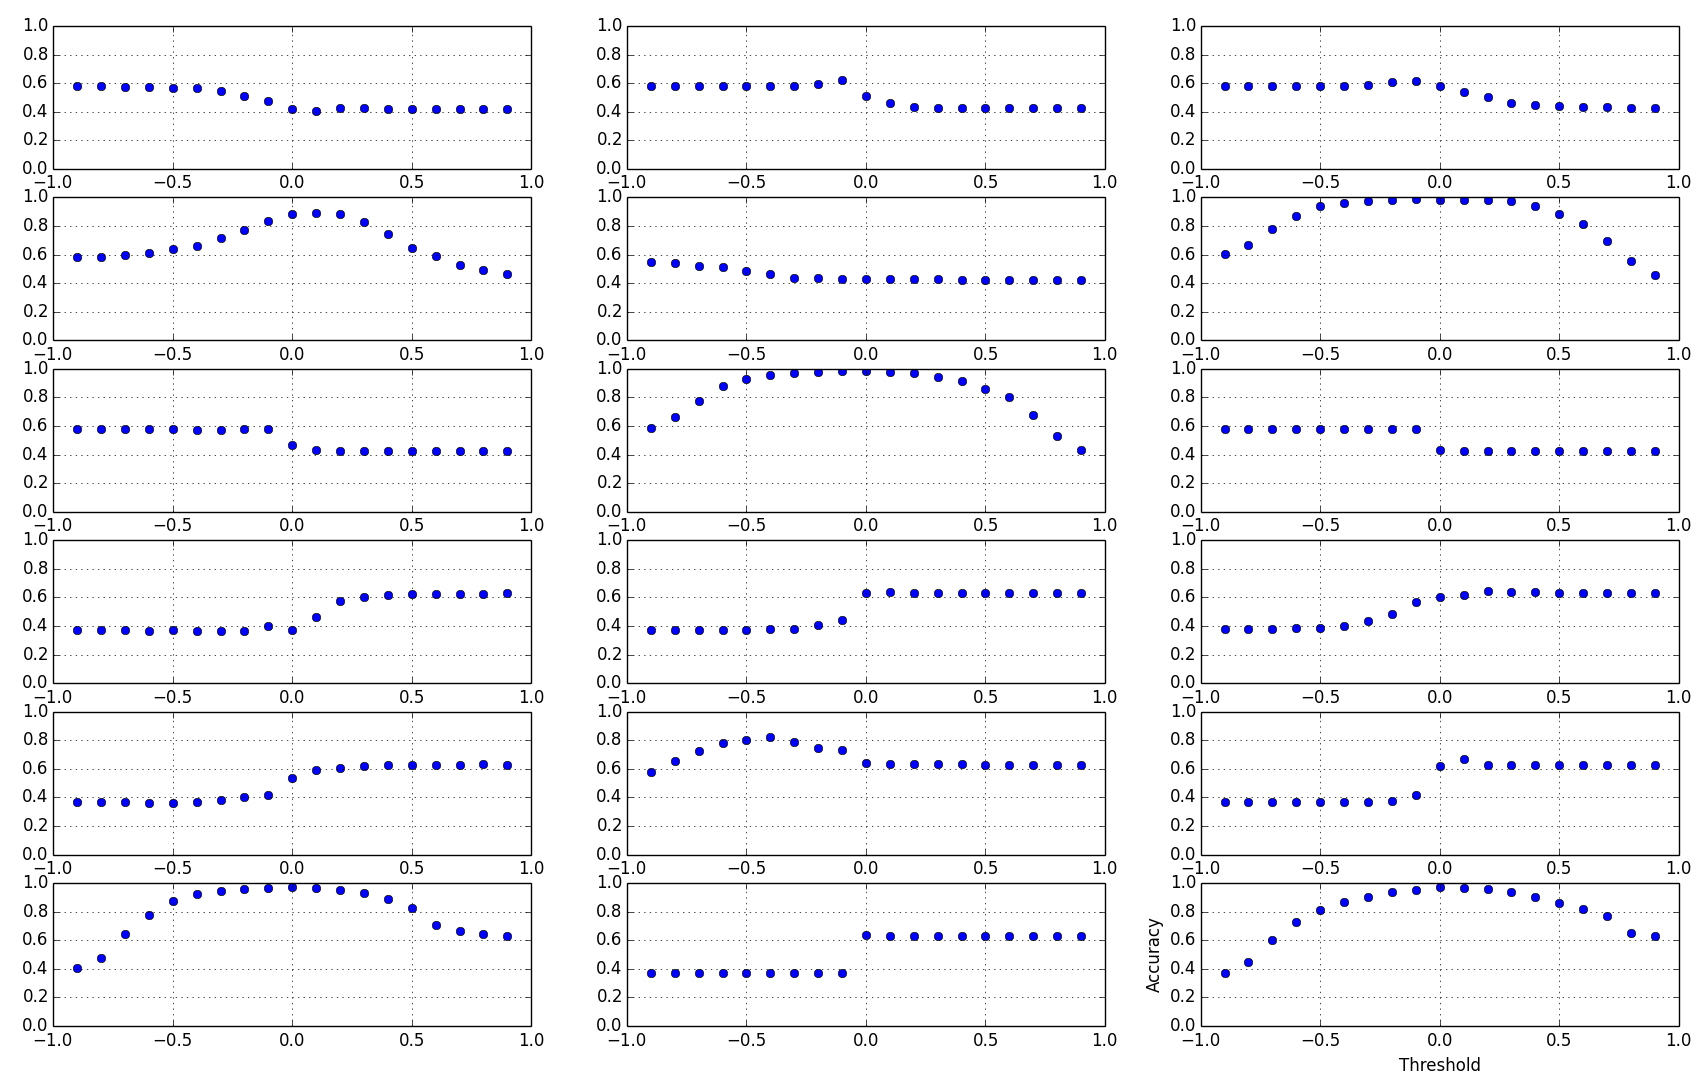
\includegraphics[width=\textwidth]{threshold_graphs.png} 
    \caption{The graphs plot the different variations of threshold. Counting is
columns first; top left is 1, top mid is 7, top right is 13.}
    \label{fig:threshold_graphs}
\end{figure}

\subsection{Drawbacks}
There are some drawbacks to the word count classification. The dictionaries
could be better and the threshold could be improved. The threshold results
depends on the dictionaries, so if we improve the dictionaries we would reduce
the threshold errors. 

\paragraph{Dictionaries}
\hspace{0pt}\\
The main drawbacks with the dictionaries are that they are based on the
datasets we classified manually. Although we cross classify so we still get
valid results. To improve the dictionaries we should expand the original
datasets and combine the dictionaries. We should also remove stop words before
creating bi and monograms.

\paragraph{Threshold}
\hspace{0pt}\\
When classifying with the word count classifier a potential problem is when we
get an equal amount of positive and negative words. Then the polarity value
becomes 0. This results in a situation where we have no indication of a tweet
being positive or negative. This is an area where we can improve the
classification. 

\begin{tabular}{ r p{6cm} r c }
id & Dictionary & Polarity=0 & Tweets \\
& -- Kiro compiled dataset -- & & \\
\hline
1 & Monogram, obama & 234 & 997 \\ 
2 & Monogram LoughranMcDonald & 543 & 997 \\ 
3 & Monogram, combined Obama and LoughranMcDonald & 178 & 997 \\
4 & Kiro, Monogram, self compiled & 53 & 997 \\
5 & Kiro, Bigram, self compiled & 7 & 997 \\
6 & Kiro, Trigram, self compiled & 28 & 997 \\
7 & Obama, Monogram, self compiled & 14 & 997 \\
8 & Obama Bigram, self compiled & 446 & 997 \\
9 & Obama Trigram, self compiled & 931 & 997 \\

& -- Obama tweet set -- & & \\
\hline
10 & Monogram, obama & 335 & 1365 \\ 
11 & Monogram LoughranMcDonald & 854 & 1365 \\
12 & Monogram, combined Obama and LoughranMcDonald & 345 & 1365 \\
13 & Kiro, Monogram, self compiled & 233 & 1365 \\
14 & Kiro, Bigram, self compiled & 462 & 1365 \\
15 & Kiro, Trigram, self compiled & 1221 & 1365 \\
16 & Obama, Monogram, self compiled & 37 & 1365 \\
17 & Obama Bigram, self compiled & 52 & 1365 \\
18 & Obama Trigram, self compiled & 92 & 1365 \\
\label{tbl:word_counting_polarity_null}
\end{tabular}

These numbers are significantly reduced if the threshold is set to 0.1.
We can also see indications that the diversity and quality of the dictionary
plays a role in the classification correctness. The more words in the
dictionary the more likely it is that we do not get an equal amount of positive
and negative words. 
%

\section{With Classifiers}\label{sentiment:classifier_classification}
To test and compare to other classification methods we used Naive Bayes and
Support Vector Machine classifiers. 

Comparing the two classifiers we found that SVM proved to be the better
classifier in this case. Although we see quite a span within the SVM results.
Details of the results and classifiers are described below.  

The self compiled dictionaries based on the kiro dataset was used to compare
the two types of classifiers. 

Each test with a classifier uses the kiro monogram dictionary for feature
extraction, and the described dataset as training set and the dataset to be
classified. 

\subsection{SVM}\label{sentiment:svm_classification}
\paragraph{Choice of kernel}
\hspace{0pt}\\
When using SVM there are quite a few different kernel modules that can be used
to improve results. The kernel is often chosen based on knowledge about the
dataset. In the nltk\footnote{Natural Language Toolkt
\url{http://www.nltk.org/}} library for python there are a number of different
kernels. We tested all of them.  

While testing which kernel was best we used the kiro dataset for training, and
the kiro monogram dictionary for feature extraction. 

Using the self compile monogram dictionaries and all the different SVM kernels we get these results:

\begin{tabular}{ l r r c }
Kernel & Failed & Correct & Accuracy \\
\hline
LinearSVC & 7 & 990 & 0.9930 \\
NuSVC & 29 & 968 & 0.9709 \\
NuSVR & 422 & 575 & 0.5767 \\
OneClassSVM & 575 & 422 & 0.4233 \\
SVC & 422 & 575 & 0.5767 \\
SVR & 422 & 575 & 0.5767 \\
\end{tabular}

Naturally we used the LinearSVC kernel later. 

\paragraph{Results}
\hspace{0pt}\\
Results from testing SVM with different dictionaries: 

\begin{tabular}{ l l r r c }
Dataset & Type & Failed & Correct & Accuracy \\
\hline
Kiro & Monogram & 7 & 990 & 0.9930 \\
Kiro & Bigram & 422 & 575 & 0.5767 \\
Obama & Monogram & 35 & 1330 & 0.9744 \\
Obama & Bigram & 507 & 858 & 0.6286 \\
\end{tabular}

From this we can draw some conclusions. The monogram dictionary performed
better than the bigram dictionary. Probably due to the number of features we
can extract from each tweet. Also classifiers are more accurate than the word
count classification method.  
%

\subsection{Naive Bayes}\label{sentiment:naive_bayes_classification}
Results from testing Naive Bayes with different dictionaries: 

\begin{tabular}{ l l r r c }
Dataset & Type & Failed & Correct & Accuracy \\
\hline
Kiro & Monogram & 29 & 968 & 0.9709 \\
Kiro & Bigram & 29 & 968 & 0.9709 \\
Obama & Monogram & 59 & 1306 & 0.9568 \\
Obama & Bigram & 59 & 1306 & 0.9568 \\
\end{tabular}

As we can see the different dictionaries makes no difference for Naive Bayes.
But if we compare the classifier with the results from the word count
classification we can clearly see improvement. 
%

\section{Comparison and Results}\label{sentiment:comparison_results}
\paragraph{The Classifiers}
\hspace{0pt}\\
We have looked at three classifiers, Naive Bayes, SVM, and the word count
classification. Together they have classified the two dataset we have with
varying results. 

All methods of classification uses the manually labeled tweet sets as the data
source. And we use the self compile dictionaries for feature extraction. 

\paragraph{The Results}
\hspace{0pt}\\
In the following table, \ref{tbl:classification_comparison}, we highlight the
results from the different classifications. We list the most noteworthy results
from our experiments and compare them.

\begin{tabular}{ l l p{3.5cm} r r c }
Classifier & Dataset & Dictionary & Failed & Correct & Accuracy \\
\hline
Word Count & Kiro & Obama Bigram & 534 & 463 & 0.4644 \\
Word Count & Obama & LoughranMcDonald Monogram & 508 & 857 & 0.6278 \\
Word Count & Obama & Kiro, Trigram & 498 & 867 & 0.6352 \\
Naive Bayes & Kiro & Kiro Monogram & 29 & 968 & 0.9709 \\
SVM & Kiro & Kiro Monogram & 7 & 990 & 0.9930 \\
\label{tbl:classification_comparison}
\end{tabular}

As we can see the classifiers give better results then the word count
classification. And SVM is a bit better than Naive Bayes. Although the results
from the word count classification indicates that the dictionaries play an
important role in the results. We can also see that monograms are better for
classifiers, while trigrams are better for word counting.

For the classifiers and the good results with the monogram dictionaries, we think
that has to do with the number of features we get from a tweet. The more
features we have the easier it is to classify and the more accurate the result. 
%

\section{Comments and Discussion}\label{sentiment:comments_discussion}
The work that is so far described potential for improvement and some
uncertainty elements. We need to address this and criticise the findings we
have.  

\subsection{Improvements}
There are a lot of improvements that could be done. 

The word count classification is merely a convenient way to say something about
the dictionaries used. We now know more about dictionaries and dictionary
compilation than we did before. But we should expand our knowledge toward the
quality of the dictionaries. And ways to eliminate terms that has no polarity
value. The dictionaries would also be greatly improved with bigger datasets to
compile the dictionaries from. 

We should cross classify and test the classification with the SVM classifier a
bit more and do quality assurance on the work with it. We should also look at
other classifiers and other data to confirm the findings we have so far. 

\subsection{Biased Mind}
The datasets of manually labeled tweets are biased based on a persons 
personal opinion and the state of mind in the moment of classification.
Therefore we have to keep in mind that all the results are based on the
assumption that everyone agrees on the manual labeling. This is of course a big
potential source of errors to be explored more in \ref{futurework}.

And we should explore the psychology of perception and classification. How do
people perceive content differently? Is finance easier to label than politics?
And what can we do to eliminate the human factor in manual labeling? 

\subsection{Drawbacks}
The drawbacks of psychology and the datasets renders some uncertainty in the
results. Although some of our observations give insight into the use of natural
language in association with dictionaries. 
Further drawbacks are the threshold of the word count classification. This
should be addressed in some smart way. 

Code wise we should improve the testing of the classifiers, and remove the
static use of dictionaries in the feature extraction.  

\subsection{Conclusions}
Dictionaries can be compiled and used in classification of sentiment. While
classifiers work better than word counting, we still rely on the manually
labeled tweets for accuracy. We also know that the data we use
to check the classification are biased and should be improved. 

\subsection{Future Work}
Analysis of the dictionaries and improvement of them would be a big task to
undertake. While we should also look at the input data and sort the data
smartly to remove spam. And find another way to decide the sentiment in the
word count classification. 

